	%% Template for ENG 401 reports
%% by Robin Turner
%% Adapted from the IEEE peer review template

%
% note that the "draftcls" or "draftclsnofoot", not "draft", option
% should be used if it is desired that the figures are to be displayed in
% draft mode.

\documentclass[peerreview]{IEEEtran}
\usepackage{cite} % Tidies up citation numbers.
\usepackage{url} % Provides better formatting of URLs.
\usepackage[utf8]{inputenc} % Allows Turkish characters.
\usepackage{booktabs} % Allows the use of \toprule, \midrule and \bottomrule in tables for horizontal lines
\usepackage{graphicx}
\usepackage{tabularx}



\usepackage[margin=10pt, labelfont=bf, format=hang, textfont={small,it}]{caption} % for more interesting captions
\captionsetup[subfigure]{style=default, margin=0pt, labelfont=bf, textfont={small,it}, singlelinecheck=true} % makes subfigure captions a bit more interesting.

\usepackage[utf8]{inputenc}
\usepackage{amsmath}

%for equal hat symbol
\usepackage{scalerel,amssymb}

\newcommand\equalhat{%
\let\savearraystretch\arraystretch
\renewcommand\arraystretch{0.3}
\begin{array}{c}
\stretchto{
    \scalerel*[\widthof{=}]{\wedge}
    {\rule{1ex}{3ex}}%
}{0.5ex}\\ 
=%
\end{array}
\let\arraystretch\savearraystretch
}
%end of equal hat symbol


%for directory visualization
\usepackage{forest}

\definecolor{folderbg}{RGB}{124,166,198}
\definecolor{folderborder}{RGB}{110,144,169}

\def\Size{4pt}
\tikzset{
  folder/.pic={
    \filldraw[draw=folderborder,top color=folderbg!50,bottom color=folderbg]
      (-1.05*\Size,0.2\Size+5pt) rectangle ++(.75*\Size,-0.2\Size-5pt);  
    \filldraw[draw=folderborder,top color=folderbg!50,bottom color=folderbg]
      (-1.15*\Size,-\Size) rectangle (1.15*\Size,\Size);
  }
}
%end directory visualization




\begin{document}
%\begin{titlepage}
% paper title
% can use linebreaks \\ within to get better formatting as desired
\title{Multiple Object Tracking Intern Report}


% author names and affiliations

\author{Hasan Atakan Bedel \\
Department of Electrical and Electronics Engineering\\
Middle East Technical University\\
}
\date{31/08/2020}

% make the title area
\maketitle
\tableofcontents
\listoffigures
\listoftables
%\end{titlepage}

\IEEEpeerreviewmaketitle





\section{Introduction}
Multiple object tracking is an essential part of the perception pipeline. In order to solve this problem many methods have been developed. My internship subject was to approach this problem using classical methods which are proposed in the master thesis provided to me. To be more precise used methods are: IMM(Interaction Multiple Model) for modeling object trajectories with different kinematic models, UKF(Unscented Kalman Filter) for nonlinear filtering of the obtained measurements and JPDAF(Joint Probability Data Association Filter) for a sophisticated data association method. I have implemented all of them in python and prepared mock data to assess their results. 



\section{Problem Definition and Approach}
The objective of multiple object tracking is to link and filter object detections across the sampled timeline. This way each object's trajectory and state estimation can be obtained. The difference between single object tracking and multiple object tracking is, later needs to associate object detections with existing tracks so that their states can be estimated correctly based on these  associted detections. 

The supplied master thesis uses UKF(Unscented Kalman Filter) to estimate the object states. Kalman filter needs a prediction model to predict the next state. In the thesis multiple kinetic models are used; Constant Velocity(CV), Constant Turn-Rate Velocity(CTRV) Model and Random Motion Model(RM). CTRV has nonlinear nature, hence the need for UKF. In order to use these different models to give only one unified estimation IMM is used.

In order to track multiple objects an data association method is required. JPDAF is used for this purpose. JPDAF is a soft data association method, meaning it does not associate the detections with existing tracks one to one. It associates all detections to all tracks based on their calculated joint association probabilities.

% An example of a floating figure using the graphicx package.
% Note that \label must occur AFTER (or within) \caption.
% For figures, \caption should occur after the \includegraphics.
% Note that IEEEtran v1.7 and later has special internal code that
% is designed to preserve the operation of \label within \caption
% even when the captionsoff option is in effect. However, because
% of issues like this, it may be the safest practice to put all your
% \label just after \caption rather than within \caption{}.
%
% Reminder: the "draftcls" or "draftclsnofoot", not "draft", class
% option should be used if it is desired that the figures are to be
% displayed while in draft mode.
%


% Note that IEEE typically puts floats only at the top, even when this
% results in a large percentage of a column being occupied by floats.
\section{Objectives}

To be honest, no clear objectives were provided in the beginning of my internship, only the master thesis. After have read the thesis and searched internet for some context I have determined the objectives myself, which were seem to be approved by my supervisor Dr. Berker Logoglu. Here is the list.
\begin{itemize}
\item Implementation of IMM, UKF, JPDAF algorithms
\item Development of an test environment for the algorithms using mock data
\item Test of the algorithms on Nuscenes dataset
\end{itemize}

\section{Project Structure}
\vspace{10px}
\begin{center}

\begin{forest}
  for tree={
    font=\ttfamily,
    grow'=0,
    child anchor=west,
    parent anchor=south,
    anchor=west,
    calign=first,
    inner xsep=7pt,
    edge path={
      \noexpand\path [draw, \forestoption{edge}]
      (!u.south west) +(7.5pt,0) |- (.child anchor) pic {folder} \forestoption{edge label};
    },
    before typesetting nodes={
      if n=1
        {insert before={[,phantom]}}
        {}
    },
    fit=band,
    before computing xy={l=15pt},
  }  
[2020 Staj
  [madeUpTracking
  	[[myHelpers]
  	 [Scenarios]
  	 [Trackers]
  	]
  ]
  [optimization
  	[[Data]
  	 [Initial Point Finder]
  	 [Optimizers]
  	]
  ]
  [scans
  ]
  [Usefull Texts
  ]
]
\end{forest}
\end{center}
\captionof{figure}{Project Structure}\label{tbl:Project Structure}

\vspace{10px}


\section{IMM-UKF-JPDAF}
In this section, I will give details about the algorithms and their implementation details with some insights I have gained.

\subsection{IMM}
IMM is used to integrate multiple kinematic models to obtain fused estimate. All used models have their own weights(mode probabilities), which determine their influence on the fused estimate. Mode probabilities are updated at each measurement time step, based on if one mode(kinematic model) were more successfull to estimate at the previous time step then the other modes.


\begin{center}

\begin{tabularx}{0.4\textwidth }{@{}p{0.2\textwidth}X@{}}
\toprule
  Notation \\
  $r_k$ & The mode at time step k \\ \\
  $z_k$ & Measured state at k\\ \\
  $x_k$ & State at k\\ \\
  $\hat{x}_k$ & State mean at k\\ \\
  $\hat{z}_k$ & State measured mean at k\\ \\
  $\hat{x}^i_k$ & State mean at k according to mode i\\\\
  $\hat{x}_k^{[i]}$ & Mixed state mean at k for mode i\\\\
  $S_k$ & State innovation matrix at k\\ \\
  $Z_k$ & The measurement at time k\\ \\
  $\mu_k^i$ & Mode probability at k\\ \\
  
 
\bottomrule
\end{tabularx}

\end{center}

\captionof{table}{IMM Notation Table}\label{tbl:IMM Notation Table}

\vspace{10px}

\subsubsection{Mixing}
At each step all the models have to mix their states with each other. This is the interaction step where IMM(Interaction Multiple Model)'s 'I' take it's name. This step helps models to stay in some bound(not formal) without diverging from each other completely.

\begin{equation}
 \mu_{k-1|k-1}^{ji} \equalhat P(r_{k-1} = j \,|\, r_{k} = i, z_{0:k-1}) 
\end{equation}

\begin{equation}
\mu_{k-1|k-1}^{ji} =
\frac
 {\pi_{ji} \; \mu_{k-1}^{j}}
 {\sum\limits_{l=1}^{N_{r}} \pi_{li} \; \mu_{k-1}^{l}}
\end{equation}

\begin{equation}
\hat{x}_{k-1|k-1}^{[i]} = \sum\limits_{j=1}^{N_{r}} \mu_{k-1|k-1}^{ji} \; \hat{x}_{k-1|k-1}^j
\end{equation}


\begin{equation}
\begin{aligned}
&P_{k-1|k-1}^{[i]} = \sum\limits_{j=1}^{N_{r}} \mu_{k-1|k-1}^{ji} \;  
[P_{k-1|k-1}^j \;+ \\ 
&( \hat{x}_{k-1|k-1}^j - \hat{x}_{k-1|k-1}^{[i]} ) \,
(\hat{x}_{k-1|k-1}^j - \hat{x}_{k-1|k-1}^{[i]})^T ]
\end{aligned}
\end{equation}



\vspace{10px}

\subsubsection{Mode Prediction Updates}
\vspace{10px}
In this part each model independently predicts the next state, which are state mean and state covariance.
\subsubsection{Mode Measurement Updates}
\vspace{10px}
Again in this part each model independently updates their state using the measurement(s) given.
\subsubsection{New Mode Probabilities}
\vspace{10px}
Here each model's mode probability is calculated. New mode probabilities are dependent on how good each model were able estimate the new state, markov chains and previous mode probabilities.
\begin{equation}
\mu_k^i = \frac
{N(Z_k; \hat{z}_{k|k-1}^i, S_k^i) \; \sum\limits_{j=i}^{N_r} \pi_{ji}\,\mu_{k-1}^j }
{\sum\limits_{l=1}^{N_r} N(Z_k; \hat{z}_{k|k-1}^l, S_k^l) \; \sum\limits_{j=1}^{N_r} \pi_{jl}\,\mu_{k-1} ^j }
\end{equation}

\subsubsection{Output Estimate Calculation}
Finally the one unified estimate is calculated based on the new calculated mode probabilities. Each model can contribute to the unified estimate proportional to their mode probability. Note that this stage does not affect any part of the algorithm, it is only used for output.
\begin{equation}
\hat{x}_{k|k} = \sum\limits_{i=1}^{N_r} \mu_k^i \, \hat{x}_{k|k}^i
\end{equation}

\begin{equation}
\begin{aligned}
&P_{k|k} = \sum\limits_{i=1}^{N_r} \mu_k^i \, 
[ P_{k|k}^i +   (\hat{x}_{k|k}^i - \hat{x}_{k|k}) \, (\hat{x}_{k|k}^i - \hat{x}_{k|k})^T]
\end{aligned}
\end{equation}


\subsection{UKF}

It is used to estimate state for non-linear prediction models. Best intuitive and formal explaination is in it's original paper \cite{MERWE00}. \\

\vspace{10px}

\begin{center}

\begin{tabularx}{0.4\textwidth }{@{}p{0.2\textwidth}X@{}}
\toprule
  Notation \\ \\
  $\hat{x}_{k-1|k-1}^i$ & i'th sigma point obtained from k-1'th step \\ \\

  
 
\bottomrule
\end{tabularx}

\end{center}

\captionof{table}{UKF Notation Table}\label{tbl:UKF Notation Table}


\vspace{10px}

\subsubsection{Unscented Transform}

First sigma points are calculated. It is like sampling near the state mean, but in a systematic and proven way. Note that $ (\sqrt{(L+\lambda) \, P_{k-1|k-1}})_i $ is the i'th column or row of the matrix inside the parentheses \cite{UKFT}. But one must stick to one choice, row or column.

\begin{equation}
\begin{aligned}
&\hat{x}_{k-1|k-1}^0 = \hat{x}_{k-1|k-1} \\
&\hat{x}_{k-1|k-1}^i = \hat{x}_{k-1|k-1} \; + &(\sqrt{(L+\lambda) \, P_{k-1|k-1}})_i  \\
& &i\in 1,...,L\\
&\hat{x}_{k-1|k-1}^i = \hat{x}_{k-1|k-1} \; - &(\sqrt{(L+\lambda) \, P_{k-1|k-1}})_{\,i-L} \\
& &i\in L+1,...,2L 
\end{aligned}
\end{equation}

\subsubsection{Prediction}
At this part each sigma points are passed through the prediction function. After that, each points are used to get the predicted state mean and covariance. The used parameter values in my implementation for the parameters presented here($\alpha, \kappa, \beta ...)$ can be found in the original paper \cite{MERWE00}.
\vspace{10px}
\begin{equation}
\begin{aligned}
&\hat{x}_{k|k-1}^i = f(\hat{x}_{k-1|k-1}^i),  \; \; i\in 0,...,2L\\
&W_s^0 = \frac{\lambda}{L + \lambda}, \; W_c^0 = \frac{\lambda}{L+\lambda} + (1-\alpha^2 + \beta)\\
&W_s^i = W_c^i = \frac{1}{2(L+\lambda)}, \; \lambda = \alpha^2 (L+\kappa) - L \\
&\hat{x}_{k|k-1} = \sum\limits_{i=0}^{2L} W_s^i \, \hat{x}_{k|k-1}^i \\
&P_{k|k-1} = \sum\limits_{i=0}^{2L} W_c^i \, [\hat{x}_{k|k-1}^i-\hat{x}_{k|k-1}]\,[\hat{x}_{k|k-1}^i-\hat{x}_{k|k-1}]^T + Q 
\end{aligned}
\end{equation}
\vspace{10px}
\subsubsection{Second Unscented Transform}
In prediction state the state covariance matrix is calculated and now it is time to find the new sigma points with respect to this new predicted state mean and covariance. Why do we need these sigma points? Reason is to make measurements on these sigma points. If the measurement function is linear than this part and next part is not necessary. Update parameters($S_k, K_k$) can be calculated using the classical kalman filter equations. This is the case with my project.
\vspace{10px}
\begin{equation}
\begin{aligned}
&\hat{x}_{k|k-1}^{*0} = \hat{x}_{k|k-1} \\
&\hat{x}_{k|k-1}^{*i} = \hat{x}_{k|k-1} \; + &(\sqrt{(L+\lambda) \, P_{k|k-1}})_i  \\
& &i\in 1,...,L\\
&\hat{x}_{k|k-1}^{*i} = \hat{x}_{k|k-1} \; - &(\sqrt{(L+\lambda) \, P_{k|k-1}})_{\,i-L} \\
& &i\in L+1,...,2L 
\end{aligned}
\end{equation}
\vspace{10px}
\subsubsection{Calculate Update Parameters}
If the measurement function is linear, which is the case for my situation, than this part can be replaced with classical kalman filter update parameter calculations. In my implementation I have coded both of them to see the difference. Note that I have not seen any formal explaination to do this but it made sense and indeed they give the exact same result.
\vspace{10px}

\begin{equation}
\begin{aligned}
&\hat{z}_k^i = h(\hat{x}_{k|k-1}^i), \; i\in 0,...,2L\\
&\hat{z}_{k|k-1} = \sum\limits_{i=0}^{2L} W_s^i \; \hat{z}_k^i \\
&P_{z_{k|k-1}, z_{k|k-1}} = \sum\limits_{i=0}^{2L} W_c^i \, [\hat{z}_{k|k-1}^i - \hat{z}_{k|k-1}]\,[\hat{z}_{k|k-1}^i - \hat{z}_{k|k-1}]^T \\
&S_k = P_{z_{k|k-1}, z_{k|k-1}} + R\\
&P_{x_{k|k-1}, z_{k|k-1}} = \sum\limits_{i=0}^{2L} W_c^i \, [\hat{x}_{k|k-1}^i - \hat{x}_{k|k-1}]\;[\hat{z}_{k|k-1}^i - \hat{z}_{k|k-1}]^T\\
&K_k = P_{x_{k|k-1},z_{k|k-1}} \; S^{-1}_k
\end{aligned}
\end{equation}

\vspace{10px}

\subsubsection{Update}
These are usual kalman filter update equations.
\begin{equation}
\begin{aligned}
&\hat{x}_k = \hat{x}_{k|k-1} + K_k \; (Z_k - \hat{z}_{k|k-1}) \\
&P_k = P_{k|k-1} - K_k \; S \; K_k^T
\end{aligned}
\end{equation}

\vspace{10px}

\subsection{JPDAF}
 JPDAF is used for soft data association. It assumes that the number of existing tracks is a known, meaning it does not have power to initiate new tracks from the given measurements. It calculates the possibility of associations between each track and each measurement. This data association probability is the output of the JPDAF. Later these probabilities are passed to PDAF along with the measurements to update the each tracker. JPDAF is clearly explained in \cite{BYL95}, but implementation part was not clear.

\vspace{10px}

\subsubsection{Validation Matrix}
"Validation Matrix" is presented here \cite[p.312]{BYL95}. It is a binary matrix with $m_k$ number of rows and $N_r+1$ number of columns. The elements of the matrix, lets say $b_{i,j}$, represent if the i'th measurement is close to j'th track. If it is close, that element is 1 otherwise 0. Whether a measurement is close to a track is decided based on the mahalonobis distance between the track's measured state mean and the measurement, using the innovation matrix as the covariance. The rationale can be find in \cite[p.312]{BYL95}. Note that $j=0$ represents the possibility of that measurement is associated with no track. To include this possibility for all measurements the first column of the validation matrix is initiated as 1.

\vspace{10px}

\subsubsection{Association Events}
An association event is nothing but just one of the possibilites to associate the existing tracks and the incoming measurements. In my implementation I have written an exhaustive algorithm($O(m_k^{N_r+1})$) to try find the possible association events using the validation matrix. If the validation matrix is dense, meaning the all measurements are close to all tracks, and if there are vast number of tracks and measurements, the performance of the algorithms is very bad. I measured the run time of my implementation with $m_k = 8$ and $N_r = 8$ and filling the validation matrix with all ones, as $41.797$ seconds, which is very bad. On the other hand with $m_k = 5$ and $N_r = 5$ and filling the validation matrix with all ones, as $0.036$ seconds. Note that a more sparse validation matrix really helps to time performance, but downside is the sparsity can not be guaranteed.

\vspace{10px}

\subsubsection{Joint Association Probabilities}
All possible events were generated and stored. Now it is time to calculate their probability. Now here I give the formal definition of an event ${\theta}$.
\begin{equation}
\begin{aligned}
\theta = \bigcap\limits_{j=1}^m \theta_{j,t_j}
\end{aligned}
\end{equation}

where $\theta_{j,t_j}$ is the event that measurement j is associated with track $t_j$. Track $t_j$ is the associated track with measurement j.

Now here are the two ways of calculating the probability of an event.
\vspace{5px}

Parametric calculation:
\begin{equation}
\begin{aligned}
P(\theta|Z^k) = \frac{1}{c} \; \prod\limits_{j=1}^{m_k} \{ \lambda^{-1} \, f_{t_j}[z_j(k)] \} ^{\tau_j} \; \prod\limits_{t=1}^{N_r} (P_D)^{\delta_t} \, (1-P_D)^{1-\delta_t}
\end{aligned}
\end{equation}

Nonparametric calculation:

\begin{equation}
\begin{aligned}
P(\theta|Z^k) = \frac{1}{c^{'}} \; \phi! \; \prod\limits_{j=1}^{m_k} \{ V \, f_{t_j}[z_j(k)] \} ^{\tau_j} \; \prod\limits_{t=1}^{N_r} (P_D)^{\delta_t} \, (1-P_D)^{1-\delta_t}
\end{aligned}
\end{equation}

\begin{equation}
\begin{aligned}
f_{t_j}[z_j(k)] = N[Z^j_k; \; \hat{z}^{t_j}_{k|k-1}, \; S^{t_j}_k]
\end{aligned}
\end{equation}

\vspace{5px}

The derivations can be found in \cite[p.317]{BYL95}.

\vspace{5px}

\begin{center}

\begin{tabularx}{0.4\textwidth }{@{}p{0.2\textwidth}X@{}}
\toprule
  Notation \\ \\
  $V$ & Volume of the surveillance region \\ \\
  $\lambda$ & Spatial density of false measurements \\ \\
  $P_D$ & Detection probability of the detector \\ \\
  $\delta_t$ & A binary number showing whether target t is associated with a measurement in that event\\ \\
  $\tau_j$ & A binary number showing whether measurement j is associated with a target in that event \\ \\
  $t_j$ & It is the index of the track which measurement j is associated with in that event \\ \\
  $\phi$ & The number of false alarms in that event\\ \\
  
 
\bottomrule
\end{tabularx}

\end{center}

\captionof{table}{JPDAF Notation Table}\label{tbl:JPDAF Notation Table}

\vspace{10px}

The implementation of surveillance region was not clear in \cite{BYL95}. One solution could be to take the volume of the track with highest volume\cite[p.211]{BYL95}, or maybe summing the max volumes of all tracks could be a solution. That is why I haven't implemented the non-parametric version, it is ambiguous. \\

Note that the calculation of event probabilities are not normalized(there is a $\frac{1}{c}$ constant in the event probability calculation). That is why we need to normalize the event probabilities now.

\begin{equation}
\begin{aligned}
P(\theta|Z^k) = \frac{P(\theta|Z^k)}{\sum\limits_{\theta^{'}\in \, all \, events} P(\theta^{'}|Z^k)}
\end{aligned}
\end{equation}

After normalization it is time to calculate the data association probabilities needed for the PDAF part. 

\begin{equation}
\begin{aligned}
\beta^{jt}_k \equalhat P(\theta_{jt}|Z_k) = \sum\limits_{\theta: \; \theta_{jt} \in \theta} P(\theta | Z_k)
\end{aligned}
\end{equation}

where $\theta_{jt}$ is the event that measurement j is associated with target t.

Equation(18) is for $j\in 1,...,m_k$. For j=0, meaning no measurement is associated with the track t, here is the calculation.
\begin{equation}
\begin{aligned}
\beta^{0t}_k = 1 - \sum\limits_{j=1}^{m_k} \beta^{jt}_k
\end{aligned}
\end{equation}


\subsection{PDAF}
PDAF is about updating a track t with multiple measurements each of which has a association probability with that track t. In fact, one of the measurements is "no measurement available for track" which also has a probability \cite[p.130]{BYL95}.\\

Note that, I will omit the superscript "t" from the equations, which would represent the equations are for track t. \\

Here are some variables to be used in the state update equations.\\
\begin{equation}
\begin{aligned}
&v^j_k = Z^j_k - \hat{z}_{k|k-1} \\
&v_k = \sum\limits_{j=1}^{m_k} \beta^{jt}_k \; v^j_k \\
&P^c_{k|k} = P_{k|k-1} - K_k \, S_k \, K_k^T \\
&\tilde{P}_k \equalhat K_k \; [\sum\limits_{j=1}^{m_k} \beta^{jt}_k \, v^j_k \, (v^j_k)^T \; - \; v_k \, v_k^T ] \; K_k^T
\end{aligned}
\end{equation}

Now the state update equations. \\

\begin{equation}
\begin{aligned}
&\hat{x}_{k|k} = \hat{x}_{k|k-1} + K_k \, v_k \\
&P_{k|k} = \beta^{0t}_k \, P_{k|k-1} + 	[1-\beta^{0t}_k] \, P^c_{k|k} + \tilde{P}_k
\end{aligned}
\end{equation}

The explanation and derivation can be find in \cite[p.130]{BYL95}.





\subsection{Putting It All Together}
I will now summarize how to use all these algorithms together. Note that only change will be in IMM algorithm in the calculation of new mode probabilities. \\

\vspace{5px}

\subsubsection{Mixings}
This part is not different. For each track, independently from other tracks, different models will mix their states based on their mode probabilities.

\vspace{10px}

\subsubsection{Predictions}
This part is not different. Each track's, independently from other tracks and independent from other models inside that track, will predict the next state using UKF algorithm.

\vspace{10px} 
 
\subsubsection{Joint Data Association Probabilities Calculation}
This part is tricky with IMM. Each track should have a state, whereas with IMM they have models. That is why for the event probability calculations one needs to fuse these models to get one state for each track. This fusing is same as the output stage of the IMM, but using the predictions of the models and the previous stage mode probabilities, at least this is what I have implemented. I could not find any information how to implement this part elsewhere.

\vspace{10px} 

\subsubsection{Updates}
In this part using the data association probabilities and measurements calculated from JPDAF stage, each track's models will update their states.

\vspace{10px}

\subsubsection{New Mode Probabilities Calculation}
This is the part where new equation is needed, since there isn't just one measurement but measurements, hence mode probability calculation must be altered. Here is the equations from \cite[p.211]{BYL95} and \cite[p.53]{AAR17}.

\begin{equation}
\begin{aligned}
\mu^i_k = \frac{\wedge^i_k[Z_k] \; \sum\limits_{j=1}^{N_r} \pi_{ji} \, \mu^j_{k-1}}{\sum\limits_{l=1}^{N_r} \{  \wedge^l_k[Z_k] \, \sum\limits_{j=1}^{N_r} \pi_{jl} \, \mu^j_{k-1} \} } 
\end{aligned}
\end{equation}


where
\begin{equation}
\begin{aligned}
\wedge^j[Z_k] = \frac{1 - P_D}{V^{m_k}} + \frac{P_D}{m_k \, V^{m_k -1}} \; \sum\limits_{i=1}^{m_k} N[Z^i_k; \, \hat{z}^j_{k|k-1}, \, S^j_k] 
\end{aligned}
\end{equation}

Note that, in my implementation I have used the highest volume among the models as the volume V, surveillance region. The volume calculation can be found here \cite[p.130]{BYL95}.

\vspace{10px}

\subsubsection{Final Output Estimations}

Each track will fuse their models using the new calculated model probabilities to get an updated estimate for their states.


\subsection{Testing of the Algorithms}
In order to verify and validate my implementation I have created mock data and implemented tracker classes to track these generated data.

\begin{figure}[htbp]
\centerline{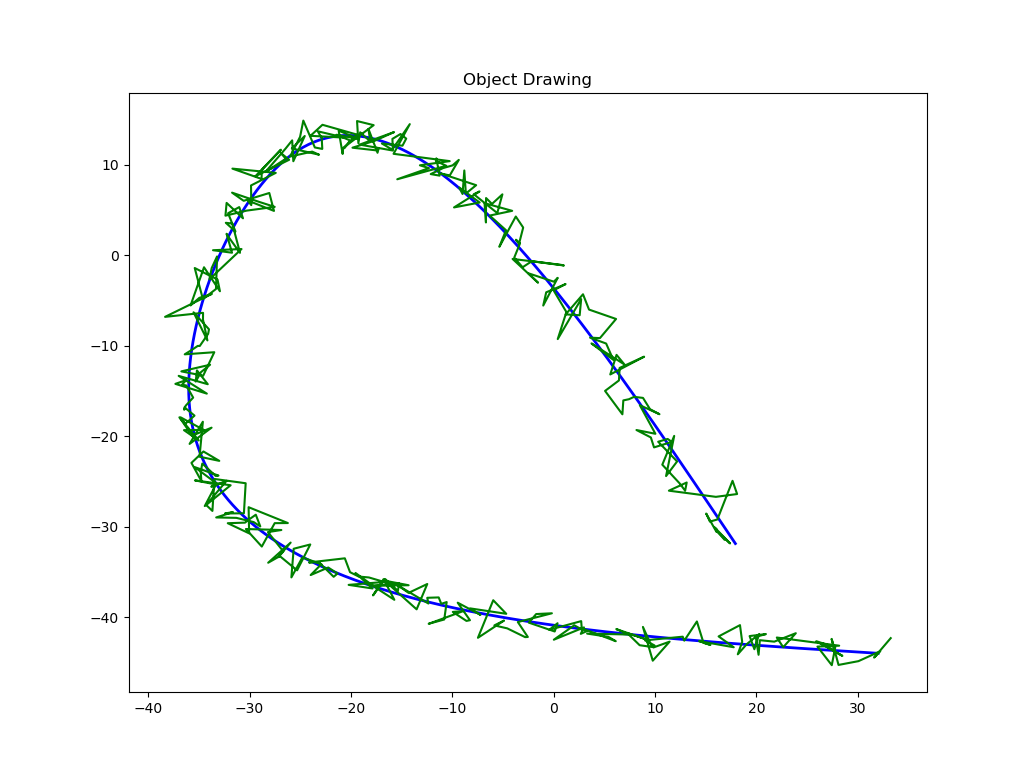
\includegraphics[scale=.3]{mockData.png}}
\caption{This is an image of a randomly generated scene. Blue path is ground truth and green lines are noisy measurements generated by adding gaussian noise added upon to the ground truth.}
\label{fig}
\end{figure}

Unfortunately, I did not have time to test them on a real data set.

\section{Trackers}
I have implemented 4 different tracker classes to test my algorithms. I have run them on randomly generated scenes to see if they actually work or how good they work.

Note that I have implemented track initialization based on the simple algorithm presented here, \cite[p.247]{BYL01}

\subsection{Single Object Single Model Tracker}

This class can be found inside "madeUpTrackers/Trackers/SingleTarget/allMe" folder. \\

It is used to track single object with single model. The measurement to be fed to the tracker in each sampling time is expected to exist and be one. Usage of this class can be found in "demo\_singleTarget.py". \\

The algorithm of the interest to be validated is \emph{UKF}. I have implemented 3 different models; Constant Velocity(CV), Constant Velocity Turn Rate(CVTR), Random Motion(RM). I have implemented CV in two different ways, both with classic kalman filter and  unscented kalman filter, since CV is a linear model. I have checked different implementations online(e.g. filterpy) to make sure I have implemented correctly. Both comparing with different implementation and testing it on mock data, I have concluded, it is correct.

\begin{figure}[htbp]
\centerline{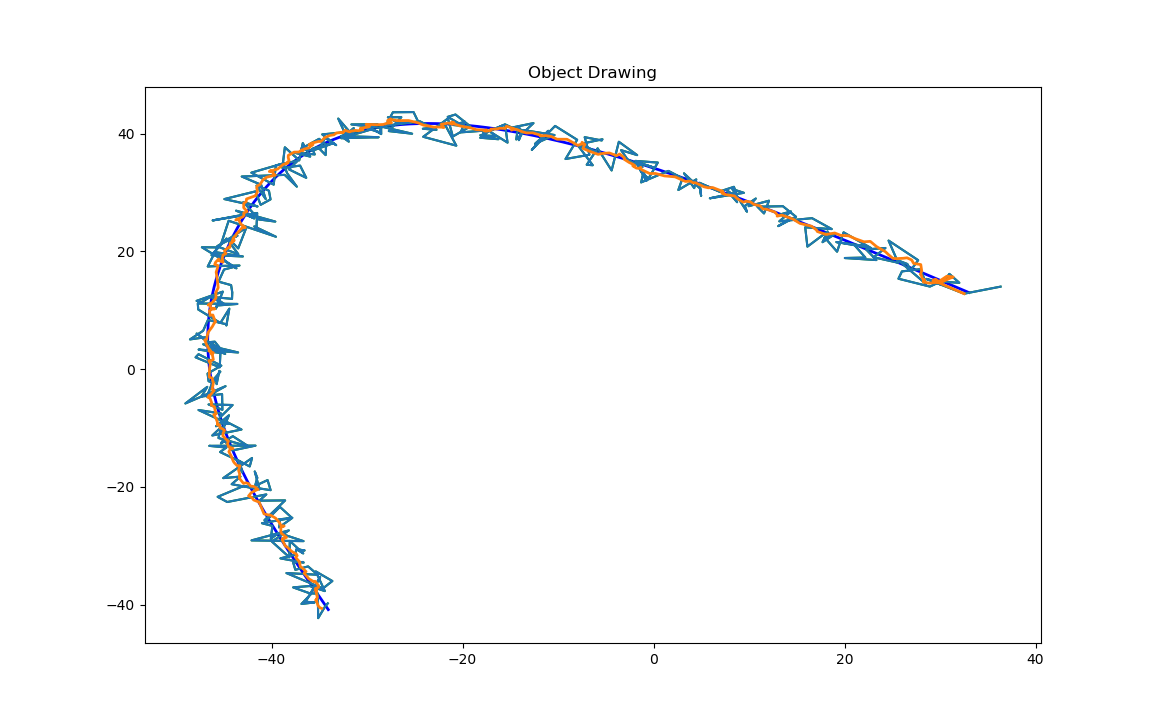
\includegraphics[scale=.3]{singleTarget_singleModel_test.png}}
\caption{This is the result of the tracking using "Single Object Single Model" tracker class with model "CV" using unscented kalman implementation on a randomly generated scene. Light blue line is measurements dark blue line is ground truth and orange line is the estimates of the tracker}
\label{fig}
\end{figure}

\subsection{Single Object Multiple Model Tracker}
This class can be found inside "madeUpTrackers/Trackers/SingleTarget/allMe" folder. \\

It is used to track single object with multiple model. The measurement to be fed to the tracker in each sampling time is expected to exist and be one. Usage of this class can be found in "demo\_singleTarget.py". \\

The algorithms of the interest to be validated are \emph{UKF} and \emph{IMM}. I have combined "CV" and "CVTR" models. Previously I have added "RM" model too, but the results were not satisfying. In the master thesis it was added, maybe after process noise optimization it would give nice results. You can change the class to add more models. Just add new model forward and measurement functions. Also you would need to change the markov chain matrix and initial mode probabilities. Make sure that sum of the initial mode probabilities add up to 1.

\begin{figure}[htbp]
\centerline{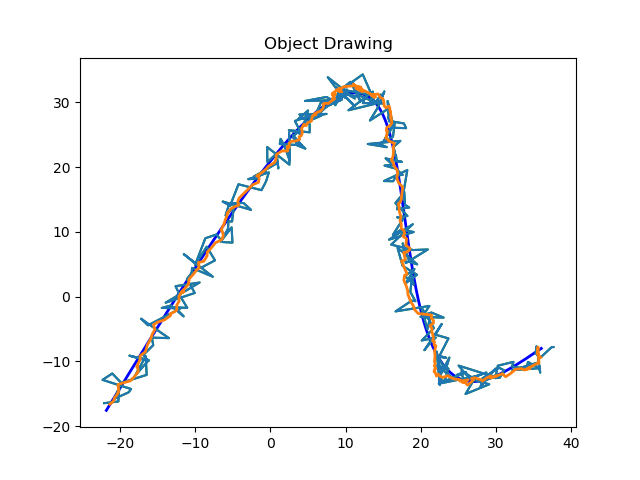
\includegraphics[scale=.5]{immPath_singleTarget.png}}
\caption{This is the result of the tracking using "Single Object Multiple Model" tracker class with models "CV" and "CVTR" combined using unscented kalman implementation on a randomly generated scene. Light blue line is measurements dark blue line is ground truth and orange line is the estimates of the tracker}
\label{fig}
\end{figure}


\begin{figure}[htbp]
\centerline{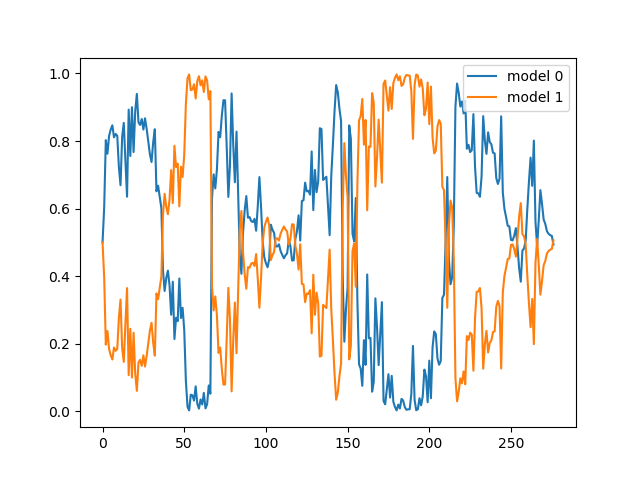
\includegraphics[scale=.5]{immProbabilities.png}}
\caption{Here are the model probabilities of the imm tracker in figure 4. The legend "model 0" corresponds to "CV" model, and "model 1" corresponds to "CVTR" model.}
\label{fig}
\end{figure}



\subsection{Multiple Object Single Model Tracker}
This class can be found inside "madeUpTrackers/Trackers/MultipleTarget/allMe" folder. \\

It is used to track multiple object with single model. The measurements to be fed to the tracker in each sampling time can be of any number, including 0. Usage of this class can be found in "demo\_multipleTarget\_singleTarget.py". \\

The algorithms of the interest to be validated are \emph{UKF} and \emph{JPDAF}. I have implemented 3 different models; Constant Velocity(CV), Constant Velocity Turn Rate(CVTR), Random Motion(RM). I have implemented CV in two different ways, both with classic kalman filter and  unscented kalman filter, since CV is a linear model. I could not find any reliable source for the JPDAF implementation. On the other hand, results on mock data indicate my JPDAF implementation is correct.

\begin{figure}[htbp]
\centerline{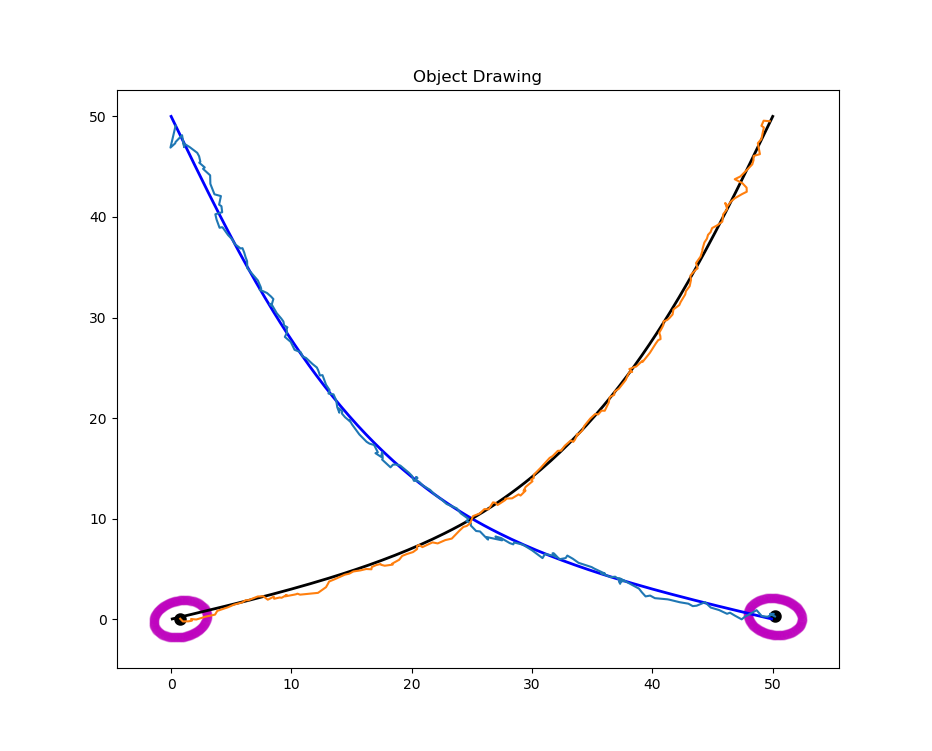
\includegraphics[scale=.3]{multiTarget_singleModel_cross.png}}
\caption{This is the result of the tracking using "Multiple Object Single Model" tracker class with model "CVTR" using unscented kalman implementation on a randomly generated scene. In this plot the measurements are not shown. Purple circles shows the gating region of the trackers, the regions where trackers are allowed to associate measurements with.}
\label{fig}
\end{figure}

\subsection{Multiple Object Multiple Model Tracker}

This class can be found inside "madeUpTrackers/Trackers/MultipleTarget/allMe" folder. \\

It is used to track multiple object with multiple model. The measurements to be fed to the tracker in each sampling time can be of any number, including 0. Usage of this class can be found in "demo\_multipleTarget\_multipleTarget.py". \\

The algorithms of the interest to be validated are \emph{UKF}, \emph{IMM} and \emph{JPDAF}. I have implemented 3 different models; Constant Velocity(CV), Constant Velocity Turn Rate(CVTR), Random Motion(RM). Although the results of imm with single target were satisfactory, this is not the case for multiple target. \\ \\ Sometimes, the predictions of the tracker increases the state covariance too much, causing the tracker to diverge. Another issue is that, there are high frequency oscillations in the tracker paths. I did not have enough time to investigate these problems. I suspect, these problems would be resolved if process noise and some other parameters in the algorithms were set right. But it could also be an implementation error, which I have checked several times and could not find.

\begin{figure}[htbp]
\centerline{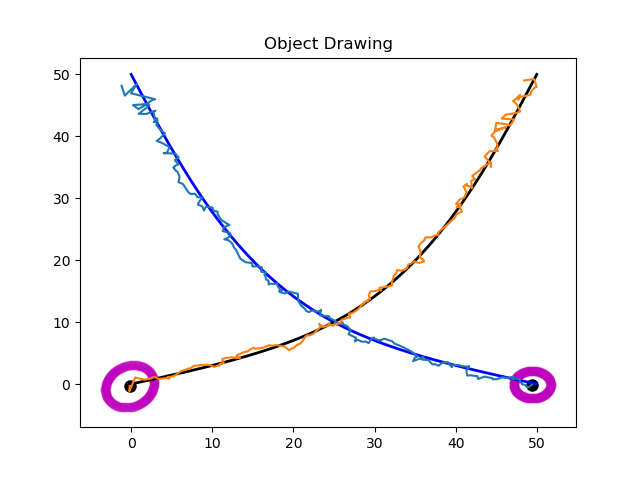
\includegraphics[scale=.4]{multiTarget_multipleModel_cross.png}}
\caption{This is the result of the tracking using "Multiple Object Multiple Model" tracker class with models "CV" and "CVTR" using unscented kalman implementation on a randomly generated scene. In this plot the measurements are not shown. Purple circles shows the gating region of the trackers, the regions where trackers are allowed to associate measurements with.}
\label{fig}
\end{figure}


\section{The Need For Optimization}
Each model needs to have a process noise matrix, which is added to the state prediction covariance matrix in every step, accounts for the model's imperfectness. If the objects to be tracked behaved exactly like the models suggest, then we would not need to add process noise, but they don't and we have to add it. \\ \\

In each iteration existing tracks' magnitude of the state covariances decreases. After few iterations their values become small enough to discard the information coming from the measurements. But if the process noise is added to these state covariances after each prediction, their magnitude does not converge to zero but to that of process noise. This way trackers don't become overconfident to discard the incoming measurements. \\ \\

Obviously, the selected values in the process noise matrix are critical. Hand picking these values can be difficult, though it is not impossible. The dynamics of the interactions between these values can give rise to counter-intuitive results that makes it hard to do. This is why one needs an optimization technique to find the best process noise possible for each models for a given data-set or environment dynamics.

\vspace{10px}

\subsubsection{Optimization}
I could not spend much time on finding the best optimization technique. Because of it's simplicity I have used the optimization technique used in [reference here] with a minor modification. \\ \\

First, I find the process noise for each model using the method given in [reference]. Then, by multiplying this matrix with scalar values selected from a interval and plotting it, I decide for the best scale for each model. At first I have tried to use back-propagation to find this best scale, but it takes to much time, and does not give me chance to see a visualization of the loss space of the complete interval. Another idea, that I have came out with is to use this scaled process noise matrix as a initial point for an back-propagation training of all the entries of the process noise. Again it took too much time to back-propagate, and I stopped working on it. If you want to work on this, make sure that with each iteration of the back-propagation, process noise matrix stays positive-definite. The way to do is generating(Cholesky decomposition) process noise from a lower or a upper triangular matrix with positive diagonal entries. While back-propagating to the lower(or upper) matrix, make sure that diagonal entries stay positive, clamp the elements of the gradient if it makes it negative. I had used the L2 distance between the updated estimates of the track and ground-truth as my loss function. \\ \\

Here is how I calculated the initial process noise covariance matrix for model "CVTR", based on the technique in [reference]. \\

First write down the model's prediction equations.
\begin{equation}
\begin{aligned}
x_{k+1|k} &= x_k + \frac{v_k}{\dot{\phi}_k} \; (-sin(\phi_k) \, + \, sin(\Delta t * \dot{\phi}_k + \phi_k )) + \boldsymbol{q_x} \\ \\
y_{k+1|k} &= y_k + \frac{v_k}{\dot{\phi}_k} \; (cos(\phi_k) \, - \, cos(\Delta t * \dot{\phi}_k + \phi_k )) + \boldsymbol{q_y} \\ \\
\phi_{k+1|k} &= \phi_k + \Delta t * \dot{\phi}_k + \boldsymbol{q_{\phi}} \\ \\
v_{k+1|k} &= v_k + \boldsymbol{q_v} \\ \\
\dot{\phi}_{k+1|k} &= \dot{\phi}_k + \boldsymbol{q_{\dot{\phi}}} 
\end{aligned}
\end{equation}

Now leave the process noises alone and find the variance of the right hand side by approximating the states using ground-truth data. Here are the approximations of the states. I will use capital letter to denote the ground truth data.\\

\begin{equation}
\begin{aligned}
&x_k \approx X_k \\ 
&y_k \approx Y_k \\ 
&v_k \approx \frac{\sqrt{(X_k - X_{k-1})^2 + (Y_k - Y_{k-1})^2}}{\Delta t} \\  
&\phi_k \approx tan^{-1}( \frac{Y_{k} - Y_{k-1}}{X_{k} - X_{k-1}}) \\ 
&\dot{\phi}_k =  \frac{\phi_k - \phi_{k-1}}{\Delta t} \\
&x_{k+1|k} \approx X_{k+1} \\ 
&y_{k+1|k} \approx Y_{k+1} \\ 
&v_{k+1|k} \approx V_{k+1} \\
&\phi_{k+1|k} \approx \phi_{k+1} \\
&\dot{\phi_{k+1|k}} \approx \dot{\phi_{k+1}} \\
\end{aligned}
\end{equation}

\vspace{5px}
\section{Performance Assesment}
\vspace{5px}

\begin{center}
\begin{tabular}{ |p{1cm}||p{2cm}|p{1.8cm}| p{1.8cm}| }
 \hline
 \multicolumn{4}{|c|}{Time Performances} \\
 \hline
 Object Count & CV(Non-linear) Model & CV(Linear) Model & IMM(CV \& CVTR)\\
 \hline
 
 3   & 209 FPS    &441 FPS& 99 FPS  \\
 4   & 152 FPS    &222 FPS& 59 FPS  \\
 5   & 75 FPS    &104 FPS& 42 FPS  \\
 7   & 22 FPS    &19 FPS& 15 FPS  \\
 
 \hline
\end{tabular}

\end{center}

\captionof{table}{Tracker Performances Table}\label{tbl:Tracker Performances Table}
\vspace{10px}
When compared, linear model is faster than non-linear model and imm. But this gap shrinks when the number of objects increases, since the over-head of JPDAF algorithms start to dominate. When the number of objects increases, performance of the trackers decreases dramatically. Main reason is that, as the objects increases, number of joint association event count increases, hence the time spent on calculation of those events. Here I give the average percentage time spent on different parts of IMM-UKF-JPDAF tracker.

\vspace{10px}
\begin{center}
\begin{tabular}{ |p{3cm}||p{1.8cm}| p{1.8cm}| }
 \hline
 \multicolumn{3}{|c|}{Spended Time on Different Parts} \\
 \hline
 Part& Average Time & Percentage\\
 \hline
 
 Prediction   & 0.013s & 8.63\%   \\ \\
 New Track Check   & 0.00113s & 0.74\%  \\\\
 Construction of Validation Matrix   & 0.000175s & 0.11\%   \\\\
 Event Generation   & 0.00732s & 4.83\%  \\\\
 Event Probability Calculations   & 0.112s & 74.50\%  \\\\
 Update   & 0.0169s & 11.16\%   \\
 
 
 \hline
\end{tabular}

\end{center}

\captionof{table}{Spended Time for tracking 8 objects with 6fps}\label{tbl:Spended Time}





\section{Fullfilment of the Objectives}
I have fulfilled my objectives partially. I have completed the implementation of the algorithms and the trackers using them step by step to test my implementations on mock data. But I could not test my trackers on a real data-set.

\section{Conclusion}
I have completed the implementation and the integration of IMM, UKF and JPDAF algorithms and successfully used them on my tracker classes. I have tried to test my implementations on mock data. I was satisfied with the results of tracker classes; "singleTarget-singleModel", "singleTarget-multipleModel", "multipleTarget-singleModel". But I am not sure if "multipleTarget-multipleModel" class is working right. The problem might be the wrong integration of IMM with JPDAF, though I have spent time to make sure it is right. Other possibility is parameters I have used are not tuned right. For this I did not spend the necessary time.


\begin{thebibliography}{1}
% Here are a few examples of different citations 
% Book
\bibitem{BYL95} 
Y. Bar-Shalom and X.-R. Li, \emph{Multitarget-Multisensor Tracking Princibles and Techniques}, 3rd~ed. 1995.

\bibitem{BYL01} 
Y. Bar-Shalom, X.-R. Li and T.Kirubarajan, \emph{Estimation with Application to Tracking and Navigation}, New York, USA: John Wiley \& Sons, Inc., 2001.


\bibitem{MERWE00} 
E. a. Wan, R. van der Merwe, and A. Nelson, “Dual estimation and the unscented
transformation,” Nips, no. January 2000, pp. 1–7, 2000.

\bibitem{AAR17} 
A.S. Abdul Rachman, 2017. 3D-LIDAR Multi Object Tracking for Autonomous Driving, Multi-target Detection and Tracking under Urban Road
Uncertainties. Delft University of Technology, Netherlands.

\bibitem{UKFT} 
Gabriel A. Terejanu. Unscented Kalman Filter Tutorial. University at Buffalo, Buffalo.




\end{thebibliography}










\end{document}